\apendice{Especificación de diseño}

\section{Introducción}

En este apartado, se van a constatar las especificaciones de diseño de este proyecto. Estas especificaciones de diseño van acorde a los objetivos propuestos al principio del proyecto y a los requisitos funcionales y no funcionales mencionados previamente. El diseño del sistema, lo podemos dividir en tres partes:

\begin{itemize}
    \item \textbf{Diseño de datos:} Define como se estructuran y almacenan los datos del sistema. Este proceso es muy importante para entender cómo se relacionan los datos y cómo definir una estructura ventajosa para el programa y sus correspondientes procedimientos.
    \item \textbf{Diseño de procedimental:} Indica los algoritmos y procedimientos utilizados en el sistema. En este proceso, suelen utilizarse los diagramas de flujo como representación gráfica de los algoritmos utilizados. 
    \item \textbf{Diseño arquitectónico:} Que el sistema posea de una buena arquitectura, es enormemente ventajoso para que sea robusto y eficiente. En este apartado se especificará cual es la arquitectura del sistema y sus principales componentes. Además, se explicarán los patrones de diseño aplicados en el proyecto.
\end{itemize}

\section{Diseño de datos}

Esta aplicación tan solo cuenta con dos entidades, las cuales son 'Convocatorias' y 'Suscripciones'. Se tomó esa decisión dado que con tan solo la creación de dos entidades se podías satisfacer los objetivos que tenía la aplicación.

Los atributos e información de interés de las correspondientes convocatorias se pueden encapsular en una sola tabla sin necesidad de relaciones con otras entidades lo cual podría suponer una pérdida de eficiencia cuando se acceden a los datos. A continuación, se va a mostrar la entidad junto con los atributos que tiene.

\imagenentidad{EntidadTFG}{Entidad Convocatorias.}

Por otro lado, para evitar que la aplicación se utilizase como herramienta de span, se limitó el número de avisos que se podían recibir por correo mensualmente. Para gestionar esto, se generó otra tabla con los emails registrados y el número de avisos que se habían enviado a ese determinado email. A continuación, se muestra gráficamente la entidad.

\imagenentidad{EntidadSuscripciones}{Entidad Suscripciones.}

\section{Diseño procedimental}

En este apartado se van a detallar los procedimientos que va a realizar un usuario al utilizar la aplicación. Para ello, se va a realizar un diagrama de flujo para indicar de manera esquematizada los distintos procedimientos y flujos que el usuario puede seguir al utilizar la aplicación. 

\newpage
\begin{landscape}
\subsection{Diagrama de flujo}
\imagenapaisada{DiagramaDeFlujo}{Diagrama de flujo.}
\end{landscape}
\newpage

\section{Diseño arquitectónico}
La arquitectura software es la encargada de diseñar la estructura que va a tener el sistema. Tener una arquitectura consistente es fundamental en aspectos de eficiencia, mantenibilidad y seguridad.

En esta fase de estructuración del sistema, juegan un papel muy importante los patrones de diseño los cuales proporcionan una mayor eficiencia y calidad de software.
Además, la utilización de estos patrones mejora la escalabilidad de los proyectos permitiendo que estos puedan crecer, pero continuando con una estructura sólida.

En este apartado, se va a comentar la arquitectura general del sistema y los patrones de diseño que han sido utilizados a lo largo del proyecto. Algunos de estos patrones han sido aplicados a la parte de \textit{web scraping} mientras que otros han sido aplicados a la hora de realizar la web. Todos los patrones utilizados, se comentarán a continuación.

\subsection{Patrones de diseño y arquitectura}

\subsubsection{Patrón de Arquitectura MVC (Modelo-Vista-Controlador)}
Este patrón ~\cite{patronmvc:latex} se utiliza para que la interfaz de usuario, los datos y la lógica de la aplicación, trabajen de manera desacoplada. Con este patrón utilizado para aplicaciones web, las solicitudes se enrutan a un controlador que es el que trabaja con el modelo de datos y, finalmente, elige la vista que se va a mostrar pasándole el modelo de datos. Más detalladamente, las capas de este patrón consisten en lo siguiente:

\begin{itemize}
    \item \textbf{Modelo:} en esta capa se encontrará una representación de los datos del dominio y la lógica de negocio de la aplicación con las que podemos gestionar entidades. El modelo es el que nos proporciona los datos que utilizamos en la aplicación y nos permite almacenarlos correctamente.
    \item \textbf{Vista:} La vista es la que se encarga de que se visualicen las interfaces de nuestra aplicación. En la vista se podrán visualizar los datos del modelo que la vista ha recibido a través del controlador.
    Para esta parte de la vista, se han utilizado las \textit{Razor Pages} dado que nos permiten incluir lógica en C\# dentro del HTML.
    \item \textbf{Controlador:} Este actúa como intermediario entre el usuario y el sistema. Este es el encargado de enviar información desde el modelo a la vista y viceversa.
\end{itemize}

\begin{figure}[H]
    \centering
    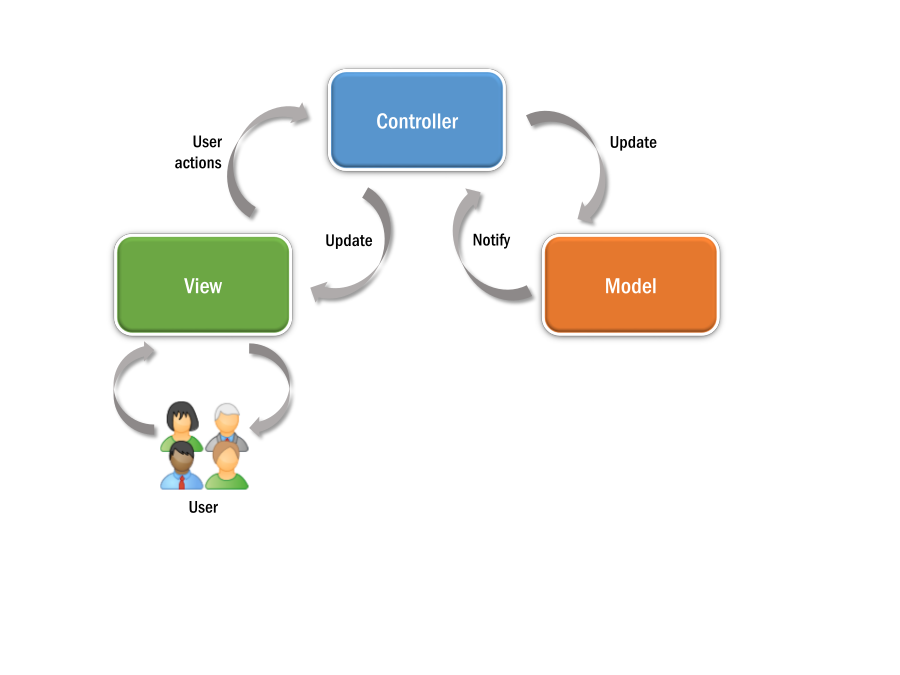
\includegraphics[width=0.9\linewidth]{DocumentacionTFG//img/PatronMVC.png}
    \caption{Patrón Modelo-Vista-Controlador ~\cite{apmvc:latex}}
\end{figure}

\subsubsection{Patrón Inyección de dependencias}

Este es un patrón de diseño admitido por .NET en el que las dependencias de una determinada clase no necesitan ser creadas si no que se inyectan directamente ~\cite{inyecciondependencias:latex}. Esto hace que las clases de alto nivel no dependan de las clases de bajo nivel.

Esto reduce el acoplamiento entre los distintos componentes de la aplicación y mejora la mantenibilidad del código.

Un ejemplo básico de utilización de este patrón en nuestra aplicación aparece cuando inyectamos el contexto de datos dentro de nuestros controladores. En lugar de generar una instancia en el propio controlador, se recibe una instancia de una determinada clase proporcionada por el contenedor de servicios donde se configuran todos los servicios que se van a utilizar en la aplicación.

\begin{figure}[H]
    \centering
    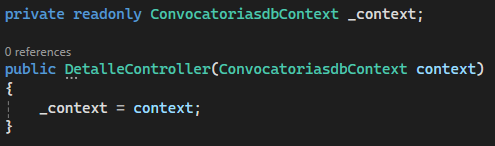
\includegraphics[width=0.7\linewidth]{DocumentacionTFG//img/InyeccionDependencias.PNG}
    \caption{Inyección de dependencias}
\end{figure}

\subsubsection{Patrón MVVM (Modelo-Modelo de Vista-Modelo)}

Este patrón aísla la vista del modelo y el modelo de la vista. La función principal del modelo de vista en este caso es proporcionar una representación de los datos que se adapte a la vista ~\cite{patronmvvm:latex}. Esto permite separar la lógica de presentación de la lógica de negocio y por lo tanto se evita que se realicen cambios importantes en el código del modelo.

En .NET este patrón se ha aplicado creando una serie de clases \textit{ViewModel} en las cuales solo se incluían los atributos que fuesen necesarios para una vista en concreto. De esta manera se evitan realizar cambios en el modelo de datos.

\begin{figure}[H]
    \centering
    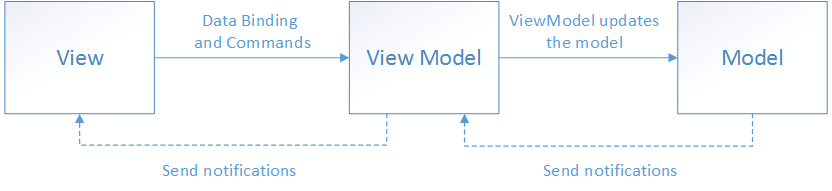
\includegraphics[width=0.9\linewidth]{DocumentacionTFG//img/PatronMVVM.png}
    \caption{Patrón MVVM}
\end{figure}

\subsubsection{Patrón Estrategia}
Este patrón se aplicó en el proceso de web \textit{scraping}, su principal propósito es permitir al objeto cliente elegir cuál de las estrategias le conviene.

En el caso del proyecto, se dispone una serie de algoritmos de \textit{scraping} en función de cada universidad. Estos algoritmos estarán cada uno en clases separadas pero todos ellos implementarán una interfaz común. Esto hace que según la universidad de la que se quiera hacer el \textit{scraping}, se selecciona su estrategia ~\cite{patronestrategia:latex}.

El patrón estrategia puede ser muy interesante de cara a futuro si se incluyen nuevas universidades en la aplicación dado que facilita enormemente las nuevas implementaciones y el testeo ~\cite{strategy:latex}.
\begin{figure}[H]
    \centering
    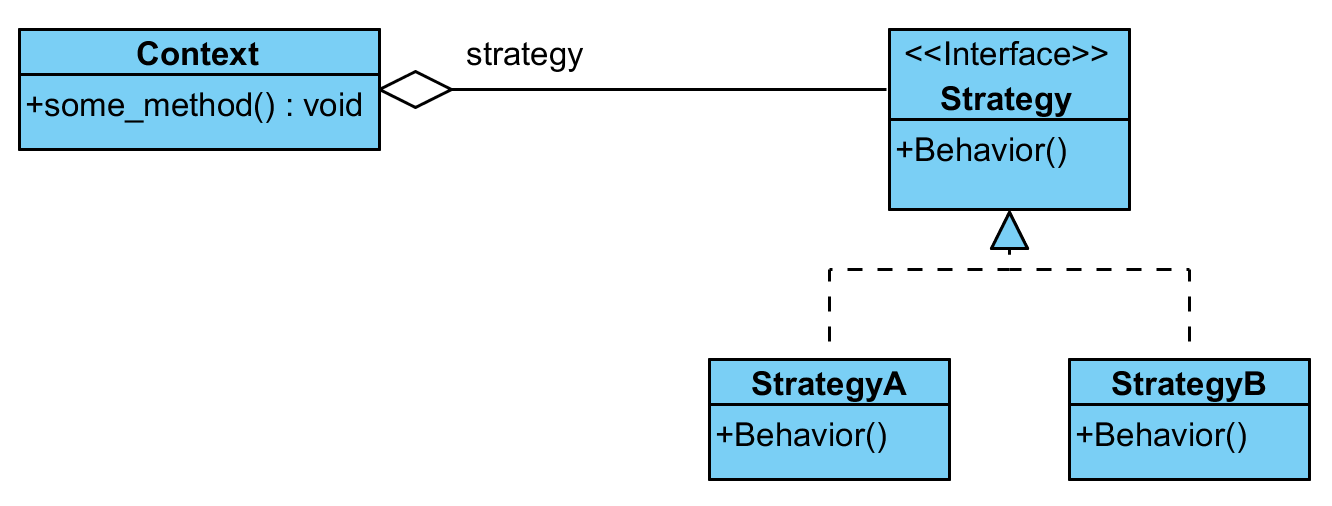
\includegraphics[width=0.7\linewidth]{DocumentacionTFG/img/PatronEstrategia.png}
    \caption{Patrón Estrategia} 
\end{figure}

\subsection{Arquitectura general del sistema}
Para lograr el objetivo de desplegar la aplicación, se tuvo que diseñar una arquitectura en la que se utilizaron distintas herramientas para desplegar los diferentes componentes del sistema. En esta apartado, se van a detallar cada una de las partes de la arquitectura del sistema tal y como se muestra gráficamente en \ref{img-diagrama-general}.

En primer lugar, he de mencionar que el sistema desarrollado tiene dos partes. Por un lado, tenemos la parte del web \textit{scraping} con Python con la que se recopilaban los datos y se actualizaba la base de datos. Por otro lado, tenemos la aplicación realizada con el \textit{framework} .NET Core MVC, esta aplicación obtiene los datos de la base de datos actualizada mediante \textit{web scraping} y los muestra en la web. Esta web es la que será utilizada por el usuario final.

Para el despliegue se ha desarrollado una arquitectura con tres componentes clave, las herramientas utilizadas se detallarán de manera más concreta en el capítulo 4 de la memoria. Aquí, se van a mencionar para un mejor entendimiento de la arquitectura.
\begin{itemize}
    \item \textbf{Servidor de Azure Database para MySQL:} En este servidor en la nube, se ha desplegado la base de datos MySQL. Esta decisión se ha tomado de esta manera debido a la facilidad que nos proporciona Azure para realizar despliegues sin realizar tareas de infraesctructura.
    \item \textbf{GitHub Action:} Esta herramienta es utilizada para la automatización de flujos de trabajo. En el sistema, se ha utilizado esta herramienta para crear una tarea programada que ejecutará el proyecto en Python y por lo tanto hará que la base de datos se actualice de manera periódica.
    \item \textbf{Azure App Services:} Este es un servicio basado en HTTP que permite hospedar aplicaciones web en la nube. En nuestro sistema, es el encargado de lanzar y alojar la aplicación desarrollada en .NET en la nube. Esto fue sencillo debido a que tanto Azure como .NET son propias de Microsoft por lo tanto el despliegue se pudo realizar con facilidad. Para que la información de la base de datos se mostrase correctamente en la web desplegada, se tuvieron que configurar las variables de entorno de este App Service e introducir la cadena de conexión de la base de datos desplegada en el servidor Azure Database. Este fue el último paso del montaje de la arquitectura del sistema y por lo tanto ya estaba la aplicación funcional disponible para utilizarse.
    \item \textbf{Usuario:} Es el encargado de interactuar con la aplicación. Para ello, accederá a la URL proporcionada por el servicio de Azure.  
\end{itemize}


\newpage
\begin{landscape}
\subsubsection{Diagrama arquitectura general del sistema}
\vspace{2cm}
\imagenapaisada{DiagramaGeneralArquitectura}{Diagrama arquitectura general del sistema.}\label{img-diagrama-general}   
\end{landscape}
\newpage


\section{Diseño de interfaces}
Dado que no había utilizado ninguna herramienta de \textit{mockup} recientemente y me parecía demasiado arcaico realizar diseños de interfaces a mano, decidí realizar los prototipos en sucio con PowerPoint. Esta decisión se tomó debido a la facilidad de uso que proporciona esa herramienta. 

Estos prototipos se fueron creando mediante la utilización de formas, contornos, fuentes, etc. A pesar de que la herramienta utilizada no es específica para realizar los prototipos, el resultado fue satisfactorio.

\begin{figure}[H]
    \centering
    \includegraphics[width=0.8\linewidth]{DocumentacionTFG//img/MaestroDiseño.png}
    \caption{Diseño Ventana Maestra}
\end{figure}

\begin{figure}[H]
    \centering
    \includegraphics[width=0.8\linewidth]{DocumentacionTFG//img/DetalleDiseño.png}
    \caption{Diseño Ventana Detalle}
\end{figure}

\begin{figure}[H]
    \centering
    \includegraphics[width=0.8\linewidth]{DocumentacionTFG//img/DiseñoAdaptativo.png}
    \caption{Diseño Adaptativo}
\end{figure}

Estos prototipos surgieron como idea inicial. Las interfaces reales se han ido modificando a medida que se iban programando para que sean más atractivas para el usuario.
